\chapter{Model-based Policy Learning}
So far we have covered the basics of model-based RL that we first learn a model and use a model for control. We have seen that this approach does not work well in general because of the effect of distributional shift in model-based RL. We have also seen the method to quantify uncertainty in our model in order to alleviate this issue. The methods we covered so far do not involve learning policies. In this chapter, we will cover model-based reinforcement learning of policies. Specifically, we will learn global policies and local policies, and combine local policies into global policies using guided policy search and policy distillation. We shall understand how and why we should use models to learn policies, global and local policy learning, and how local policies can be merged via supervised learning into a global policy.

We have seen the difference between a closed-loop and open-loop controller. We also discussed why an open-loop controller is suboptimal because we are rolling out a whole sequence of actions solely based on one state observation. Therefore, it would be more ideal if we could design a closed-loop controller where state feedbacks can help us correct the mistakes we make. Recall in a stochastic environment, we are optimizing over the policy as follows:
\begin{align*}
    p(s_1,a_1,\dots,s_T,a_T)&=p(s_1)\prod_{t=1}^T\pi(a_t|s_t)p(s_{t+1}|s_t,a_t)\\
    \pi&=\argmaxA_\pi \mathbb{E}_{\tau\sim p(\tau)}\left[\sum_t r(s_t,a_t)\right]
\end{align*}
and $\pi$ could take several forms: $\pi$ can be a neural net, which we call a \textbf{global} policy, and it can also be a time-varying linear controller $K_t s_t + k_t$ as we saw in LQR, which we call a \textbf{local} policy.

\section{Back-propagate into the Policy}
Let us start with a simple solution for model-based policy learning. Ideally, we could build a computational graph in Tensorflow, and calculate the partial derivatives step by step so that we can backpropage into policy and optimize the policy, illustrated in Fig. \ref{fig:poliback}.
\begin{figure}
    \centering
    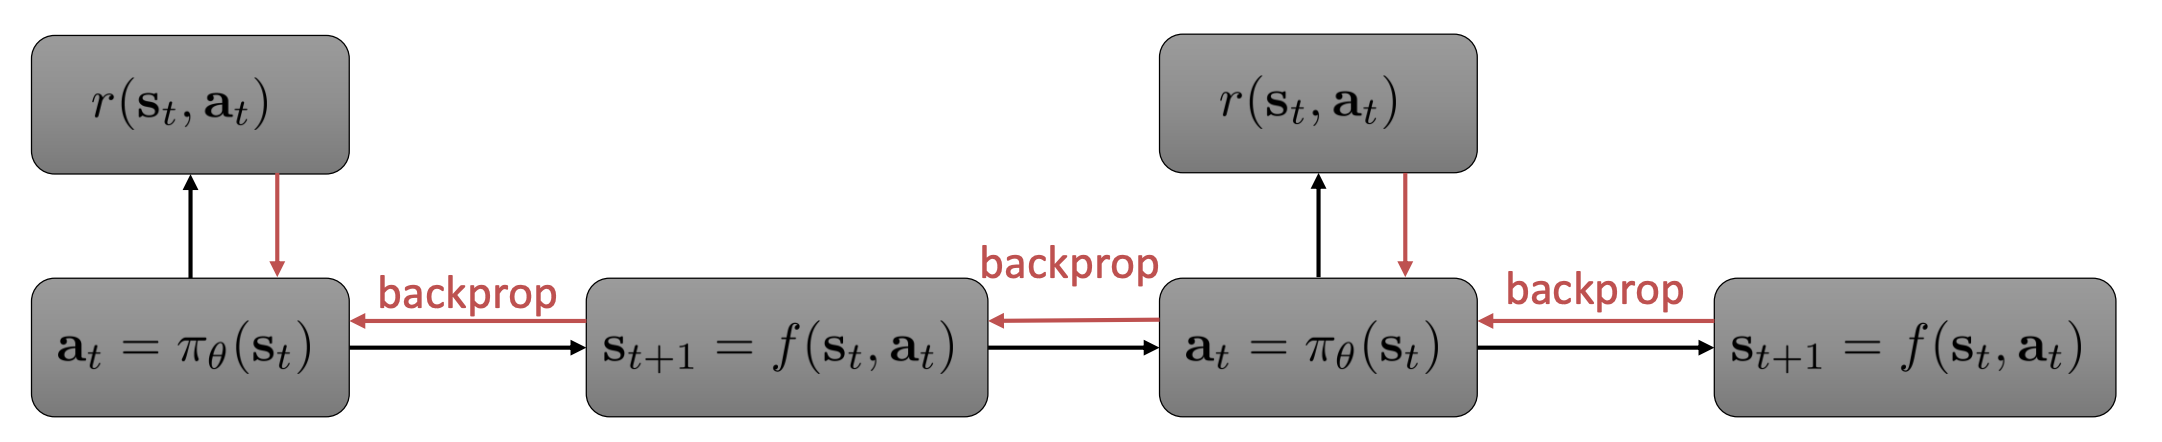
\includegraphics[scale=0.4]{figures/poliback.png}
    \caption{Back-propagate into policies}
    \label{fig:poliback}
\end{figure}
Then we can modify our model-based policy-free RL algorithm to accomodate this new policy learning process in Alg. \ref{alg:mb20}.
\begin{algorithm}[t!]
\caption{Model-based Reinforcement Learning Version 1.5}
\begin{algorithmic}[1]
\label{alg:mb20}
\REQUIRE Some base policy for data collection $\pi_0$
\STATE Run base policy $\pi_0(a_t|s_t)$ (e.g. random policy) to collect $\mathcal{D} = \{(s,a,s')_i\}$
\WHILE{True}
\STATE Learn dynamics model $f(s,a)$ to minimize $\sum_i\lvert|f(s_i,a_i)-s'_i|\rvert^2$
\STATE Backpropagate through $f(s,a)$ into the policy to optimize $\pi_\theta(a_t|s_t)$
\STATE Run $\pi_\theta(a_t|s_t)$, appending the visited tuples $(s,a,s')$ to $\mathcal{D}$.
\ENDWHILE
\end{algorithmic}
\end{algorithm}
\subsection{Vanishing and Exploding Gradients}
One problem with Alg. \ref{alg:mb20}, or general gradient-based optimization is that as we progress into the time steps, we might encounter vanishing or exploding gradients. Because as we apply chain rule, the gradients get multiplied by each other, so we the product may get extremely big (exploding) or extremely small (vanishing), making optimization a lot harder. Furthermore, we have similar parameter sensitivity problems as shooting methods, but we no longer have convenient second order LQR-like method, because the policy function is extremely complicated and policy parameters couple all the time steps, so no dynamic programming. % what does this mean

So what can we do about it? First, we can use model-free RL algorithms with synthetic samples generated by the model. Essentially, we are using models to accelerate model-free RL. Second, we cam use simpler policies than neural nets such as LQR, and train local policies to solve simple tasks, and then combine them into global policies via supervised learning. 

\section{Model-free Optimization with a Model}
Recall the equation from policy gradients:
\[
\nabla_\theta J(\theta) \simeq \frac{1}{N}\sum_{i=1}^N\sum_{t=1}^T\nabla_\theta \log\pi_\theta(a_{i,t}|s_{i,t})\hat{Q}^\pi_{i,t}
\]
Note that we are not doing any backprop through time in policy gradient because we are calculating the gradient with respect to an expectation, so we can just take the derivative of the probability of the samples instead of the actual dynamics function. 

Then we look at the regular backprop (pathwise) gradient, we see a more chain rule-like gradient:
\[
\nabla_\theta J(\theta) = \sum_{t=1}^T\frac{dr_t}{ds_t}\prod_{t'=2}^t\frac{d{s_{t'}}}{da_{t'-1}}\frac{da_{t'-1}}{ds_{t'-1}}
\]
The two gradients are different, because the policy gradient is for stochastic systems while the backprop policy is for deterministic systems. But using variational inference, we can prove that they are calculating the same gradient differently, this having different tradeoffs. We will talk about variational inference more in-depth in the next chapter. 

Actually, given more samples to reduce variance, policy gradient is more stable because it does not require multiplying many Jacobians. However, if our models are inaccurate, the samples we use from the wrong model will be incorrect, and the mistakes are likely to exacerbate as time goes on. So it would be nice to use such model-free optimizer and keep the rolled out samples' trajectory short. This is essentially what Dyna algorithm does.

\subsection{Dyna}
Dyna is an online Q-learning algorithm that performs model-free RL with a model. 
\begin{algorithm}[t!]
\caption{Dyna}
\begin{algorithmic}[1]
\label{alg:dyna}
\REQUIRE Some exploration policy for data collection $\pi_0$
\STATE Given state $s$, pick action $a$ using exploration policy
\STATE Observe $s'$ and $r$, to get transition $(s,a,s',r)$
\STATE Update model $\hat{p}(s'|s,a)$ and $\hat{r}(s,a)$ using $(s,a,s')$
\STATE Q-update: $Q(s,a)\leftarrow Q(s,a) + \alpha\mathbb{E}_{s',r}\left[r + \max_{a'} Q(s',a')-Q(s,a)\right]$
\FOR{$K$ times}
\STATE Sample $(s,a)\sim \mathcal{B}$ from buffer of past states and actions
\STATE Q-update: $Q(s,a)\leftarrow Q(s,a) + \alpha\mathbb{E}_{s',r}\left[r + \max_{a'} Q(s',a')-Q(s,a)\right]$
\ENDFOR
\end{algorithmic}
\end{algorithm}
In step 3 of Alg. \ref{alg:dyna}, we are updating the model and reward function using the observed transition. Then in step 6, we will sample some old state and action pairs and apply the model onto the sampled pair. Intuitively, as the models get better, the expectation estimate in step 7 also gets more accurate. This algorithm seems arbitrary in many aspects, but the gist is to keep improving models and use models to improve Q-function estimation by taking expectations. 

We can also generalize Dyna to see how this kind of general Dyna-style model-based RL algorithms work. The generalized algorithm is shown in Alg. \ref{alg:dynagen} \ref{alg:dynagen}.
\begin{algorithm}[t!]
\caption{General Dyna}
\begin{algorithmic}[1]
\label{alg:dynagen}
\REQUIRE Some exploration policy for data collection $\pi_0$
\STATE Collect some data, consisting of transitions $(s,a,s',r)$
\STATE Learn model $\hat{p}(s'|s,a)$ (and optionally, $\hat{r}(s,a)$
\FOR{$K$ times}
\STATE Sample $s\sim \mathcal{B}$ from buffer
\STATE Choose action $a$ (from $\mathcal{B}$, from $\pi$, or random)
\STATE Simulate $s'\sim\hat{p}(s'|s,a)$ (and $r=\hat{r}(s,a)$)
\STATE Train on $(s,a,s',r)$ with model-free RL
\STATE (optional) take $N$ more model-based steps
\ENDFOR
\end{algorithmic}
\end{algorithm}
\begin{figure}
    \centering
    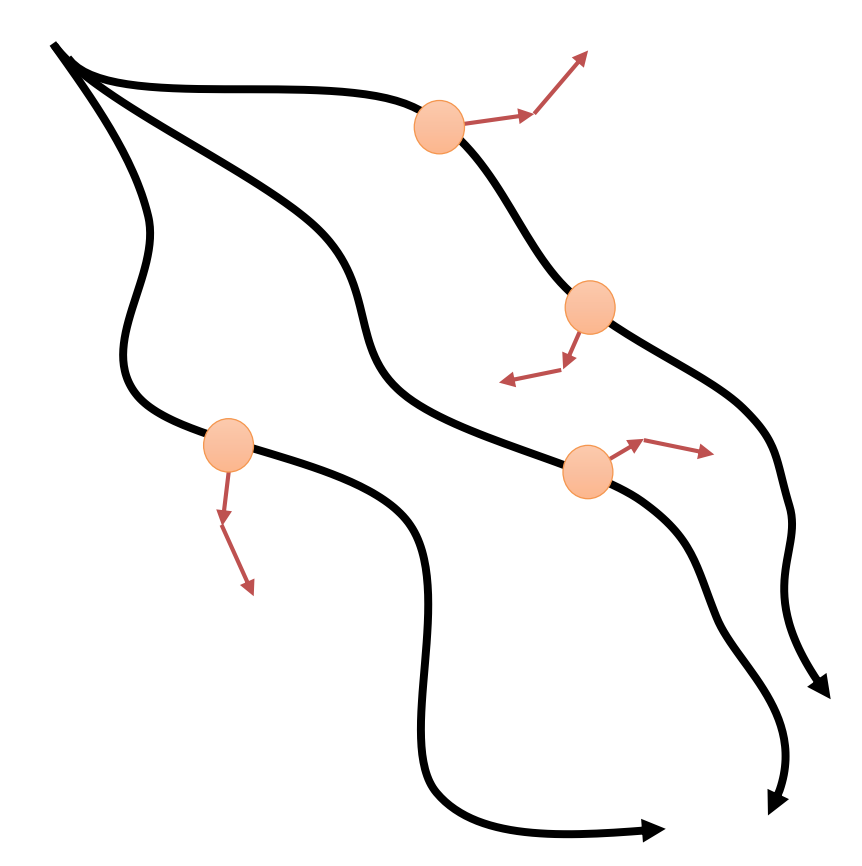
\includegraphics[scale=0.4]{figures/dynarollout.png}
    \caption{General Dyna training}
    \label{fig:dynarollout}
\end{figure}
As shown in Fig. \ref{alg:dynagen}, we choose some states (orange dots) from the buffer, simulate the next states using the learned model, and then train model-free RL with synthetic data $(s,a,s',r)$ where $s$ is from the experience buffer, $s'$ is from the learned model. One could also take more than one step if one believes that the model is good enough for more steps. 

This algorithm only requires very short (as few as one step) rollouts from model, so the mistakes will not exacerbate and accumulate much. Moreover, we explore well with a lot of samples because we still see diverse states. 

\section{Local and Global Models}
Recall that in LQR, we can turn a constrianed optimization problem into an unconstrained problem:
\[
\min_{u_1,\dots,u_T}c(x_1,u_1)+c(f(x_1,u_1),u_2)+\dots+c(f(f(\dots)\dots),u_T)
\]
Backpropagation is indeed a possible solution to solve this optimization problem, and we need $\frac{df}{d{x_t}}$, $\frac{df}{du_t}$, $\frac{dc}{dx_t}$, $\frac{dc}{du_t}$

\subsection{Local Models}
Since LQR gives us a state-feedback controller for a linear system, we can keep linearizing the system and iteratively apply LQR to generate local models. We fit $\frac{df}{d{x_t}}$, $\frac{df}{du_t}$ around the current trajectory or policy. Say the model is a Gaussian $p(x_{t+1}|x_t,u_t)=\mathcal{N}(f(x_t,u_t),\Sigma)$, then we can approximate the model as a linear function $f(x_t,u_t)\simeq A_t x_t+B_tu_t$, and we can use $\frac{df}{d{x_t}}$ as $A_t$, and $\frac{df}{du_t}$ as $B_t$.

Iterative LQR produces $\hat{x_t},\hat{u_t},K_t,k_t$, where $u_t = K_t(x_t-\hat{x_t})+k_t+\hat{u_t}$. We can execute the controller using a Gaussian $p(u_t|x_t) = \mathcal{N}(K_t(x_t-\hat{x_t})+k_t+\hat{u_t},\Sigma_t)$ because we can add noise to the iLQR controller so that all samples do not look the same. Practically, we can set $\Sigma_t = Q^{-1}_{u_t,u_t}$.
\begin{figure}
    \centering
    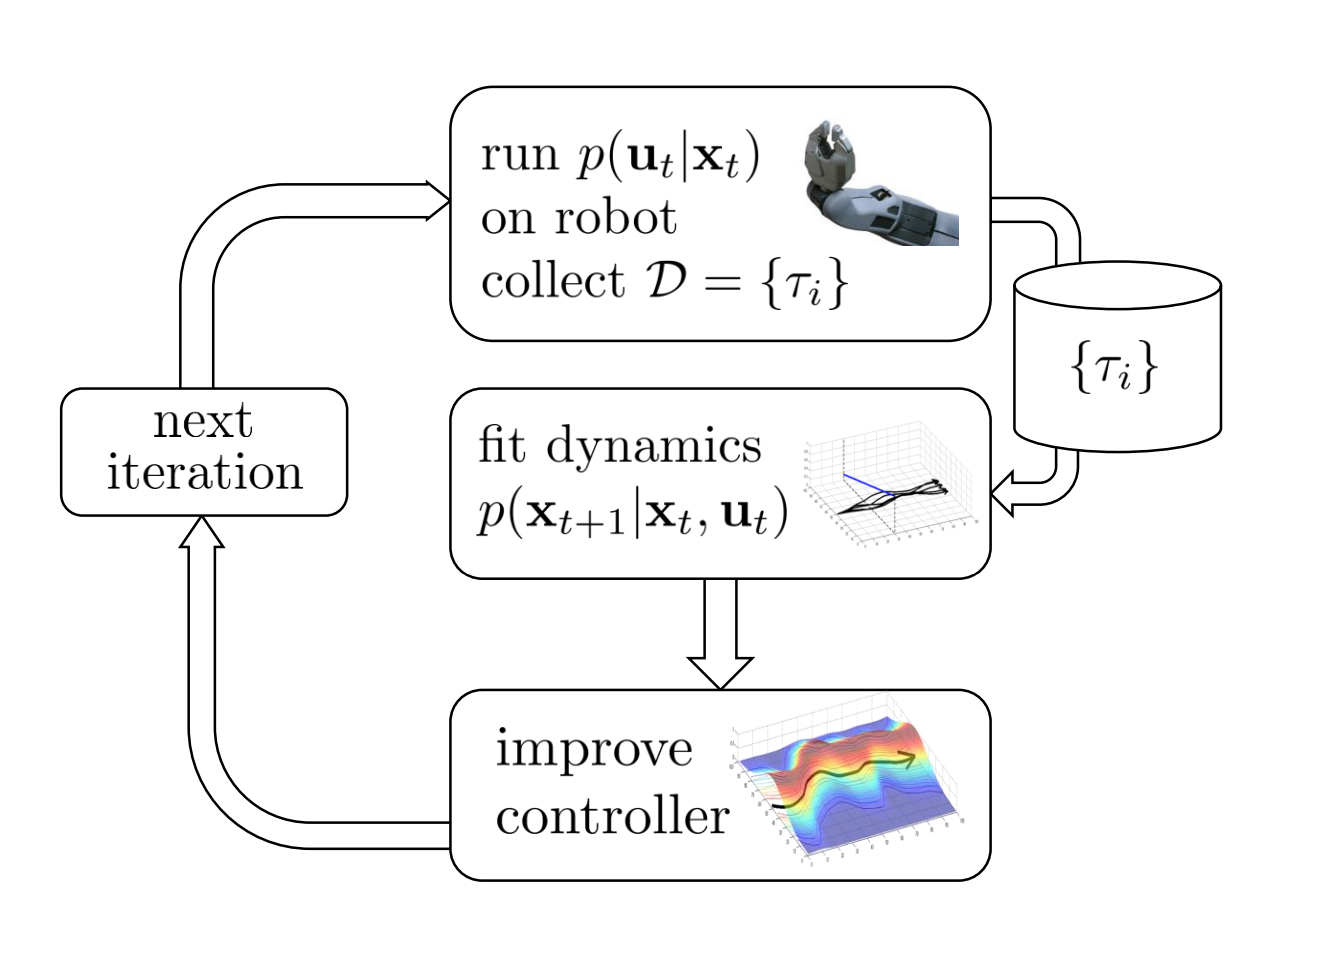
\includegraphics[scale=0.35]{figures/localmodel.png}
    \caption{Local models fitting}
    \label{fig:localmodel}
\end{figure}
We can fit the model $p(s_{t+1}|s_t,a_t)$ using Bayesian linear regression, and use the global model as prior.

We also need to stay close to old controller if we go too far. If trajectory distribution is close, then dynamics will be close too. Close here means the KL-divergence is small $D_{KL}(p(\tau)||p(\Bar{\tau}))\leq \epsilon$.

%todo: idk how fitting the dynamics works

\subsection{Guided Policy Search}
The high level idea of guided policy search is to use some simpler local policy such as local LQR controller to help and guide the learning process of more complex global policy learner. Essentially, we would use the local models trajectories as the training data for a supervised learning neural net that can solve all the tasks.

However, one problem is that the local policies might not be able to be reproduced using a single neural net. Therefore, after training the global policy with supervised learning, we need to reoptimize the local policies using the global policy so that the policies are consistent with each other. The sketch of guided policy search is shown in Alg. \ref{alg:guided}. Note that the cost function $\Tilde{c}_{k,i}$ is the modified cost function to keep $\pi_{LQR}$ close to $\pi_\theta$.
\begin{algorithm}[t!]
\caption{Guided Policy Search}
\begin{algorithmic}[1]
\label{alg:guided}
\WHILE{True}
\STATE Optimize each local policy $\pi_{LQR,i}(u_t|x_t)$ on initial state $x_{0,i}$ with respect to $\Tilde{c}_{k,i}(x_t,u_t)$
\STATE Use samples from the previous step to train $\pi_\theta(u_t|x_t)$ to mimic each $\pi_{LQR,i}(u_t|x_t)$
\STATE Update cost function $\Tilde{c}_{k+1,i}(x_t,u_t) = c(x_t,u_t) + \lambda_{k+1}\log \pi_\theta(u_t|x_t)$
\ENDWHILE
\end{algorithmic}
\end{algorithm}

In Divide and Conquer RL, the idea is similar, except that we are replacing the local LQR controllers with local neural net. 
